\chapter{Implementation} \label{chap:System_implementation}
\textit{This chapter describes the implementation of the systems we designed and discusses the applied technology.}

\minitoc

\section{The Library}
\bigskip
{\textbf{Typescript}}

TypeScript is a strict superset of javascript, designed as a strongly typed programming language by Microsoft. A strongly typed language is more secure because it requires explicit declarations to convert or compare between types in order to convert between languages. This allows for the avoidance of errors and memory exploitations such as the CWE-704 Incorrect Type Conversion or Cast \cite{cwe}. At the same time, it checks types at compile time to find any potential type errors before they are propagated into the program.

TypeScript uses a transpiler, a source-to-source compiler that takes TypeScript source and converts it into JavaScript. The TypeScript code ends up running as JavaScript. In conclusion, TypeScript does provide a set of constraints regarding typing, which enforces a higher level of security.

\bigskip
{\textbf{Tweetnacl-js}}

TweetNaCl-js is a translation of TweetNaCl to JavaScript, which is as close as possible to the original C implementation. It provides public key and secret key authenticated encryption, scalar multiplication, digital signatures, hashing, random bytes generation, and constant-time comparison. Tweetnacl was written by many cryptography experts.

Bernstein et al. \cite{Bernstein2012} focuses on the security analysis of the NaCl cryptographic library.
More specifically, the security impact of NaCl's design features, such as no data flow
from secrets to load addresses, no data flow from secrets to branch conditions; no padding oracles; centralizing randomness; avoiding unnecessary randomness; extremely high speed; and cryptographic primitives chosen conservatively in light of the cryptanalytic literature, were evaluated. Hence, these features result in a high-security cryptographic and bug-free library.

\subsection{Library core}
Our library expands on the implementation of the secp256k1 curve and their blockchain transaction problem. For the sake of our thesis, we will only present the core function of the ed25519 blockchain since others will follow the same schemas and rules (just different dependencies).

\bigskip
{\textbf{Structure}}

Applying our design with Typescripts, we have the library model as \autoref{fig:type_lib}

\begin{figure}[ht!]
    \centering
    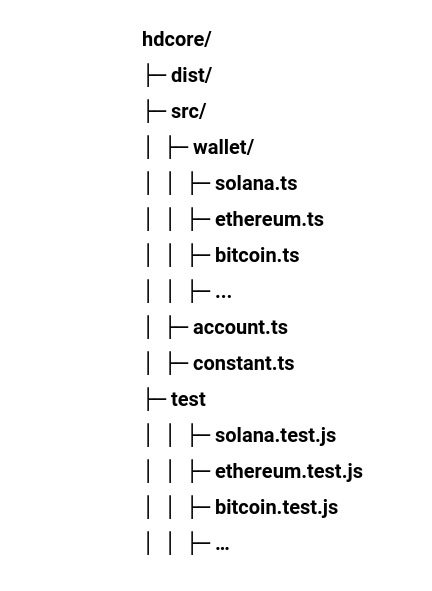
\includegraphics[width=0.5\textwidth]{images/lib_typescript.png}
    \caption[Typescript library structure]{Typescript library structure}
    \label{fig:type_lib}
\end{figure}

We design our work for developers who only use it for one specific blockchain or implement multiple of them. We also acknowledge that every blockchain has different features (especially in transactions). For example, Bitcoin uses the UTXO model (individual coins) for wallet assets, while Solana uses the Account/Balance model. This led to different implementations in transaction functions. Aiming for upgradeability, readability, and ease of use, we organized as follow:


\begin{itemize}
    \item We create a \textit{COMPONENTS} JSON object (see \autoref{fig:comp}) with constant information of every supported blockchain in \autoref{fig:ubl}. This \textit{COMPONENTS} belongs to file \textit{/src/constant.ts} (.ts is the standard for Typescript file). We made use of the JSON architecture for legibility. Users can see right away what function a blockchain has and how to access them through a few lines of code. Unlike  Tomi Jaga's wallet \cite{tomi}, they use an OOP structure which is very hard to read. Also, it would become more redundant when we created more blockchain dictionaries and added more features for each of every blockchain. Meanwhile, in our JSON object, developers can add more lines with different indexes and add the new function to their blockchain file (solana.ts, etc.).
          \begin{figure}[ht!]
              \centering
              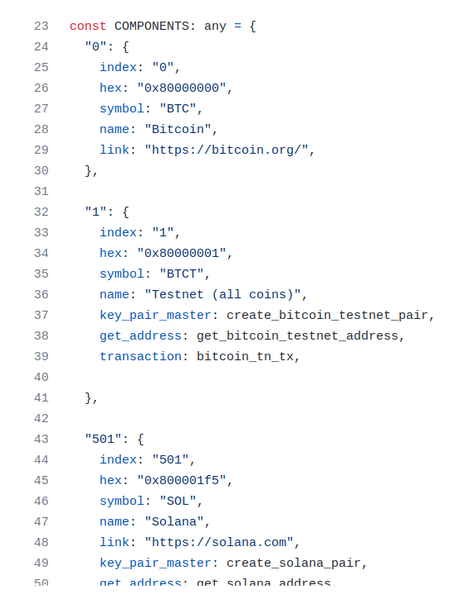
\includegraphics[width=0.5\textwidth]{images/components.png}
              \caption[COMPONENTS JSON example]{COMPONENTS JSON example}
              \label{fig:comp}
          \end{figure}
    \item For the users who want to implement the functions generally, we create \textit{/src/accounts.ts} for this purpose. It includes the function to access these values and supports every element of the key derivation process. We present it in the library API part (see Section \ref{typeapi}).
\end{itemize}

\subsection{Important dependencies}

To handle curve ed25519 arithmetic, we use the tweetnacl-js library as mentioned. The library uses Asymmetric Cryptography in NaCl that applied Bernstein's Curve25519 elliptic-curve Diffie-Hellman key exchange and will use the Ed25519 elliptic-curve signature scheme from Bernstein, Duif, Lange, Schwabe, and Yang as presented in Section \ref{cryptography}. One thing is different; they didn’t use the principle as we have shown for scalar multiplication with the ed25519 curve. They decided not to implement the conversion of points on ed25519 to Montgomery form and back. Instead, they perform a new ladder with a completely new addition and double points in one add function. The pseudo-code describes as in \autoref{fig:implement_sign_lib}:
\begin{figure}[ht!]
    \centering
    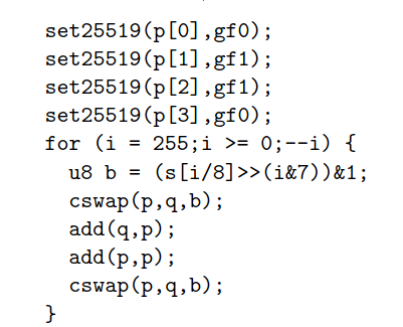
\includegraphics[width=0.4\textwidth]{images/signnaclpart.png}
    \caption[Different implementation in Montgomery Ladder]{Different implementation in Montgomery Ladder}
    \label{fig:implement_sign_lib}
\end{figure}

\subsection{Library API}
\label{typeapi}
The main API are listed as:
\begin{itemize}
    \item \textbf{hdcore.account.createMnemonic()}
          \begin{quote}
              Return a mnemonic code with 12 or 24 words.
          \end{quote}

    \item \textbf{hdcore.account.createSeed()}
          \begin{quote}
              Return a master seed with 512 bits.
          \end{quote}

    \item \textbf{hdcore.account.createMasterAccount()}
          \begin{quote}
              Return a master private key and public key.
          \end{quote}

    \item \textbf{hdcore.account.getPath()}
          \begin{quote}
              Return BIP44 path (note that we only test with depth = 7). We also provided getFullPath function for who want to create longer path.
          \end{quote}

    \item \textbf{hdcore.account.createChildAccount()}
          \begin{quote}
              Return child account with a specific path.
          \end{quote}

    \item \textbf{hdcore.account.getTransaction()}
          \begin{quote}
              Return the \textbf{transaction} object, which has some functions below.
          \end{quote}

    \item \textbf{transaction.airdrop\_one()}
          \begin{quote}
              Request airdrop on testnet/devnet.
          \end{quote}

    \item \textbf{transaction.get\_balance()}
          \begin{quote}
              Request get balance of an account (for account-based blockchain).
          \end{quote}

    \item \textbf{transaction.send()}
          \begin{quote}
              Broadcast transaction to the networks.
          \end{quote}
\end{itemize}

A few more function supports every detail to make the wallet work appropriately (for example, address validation, public key validation, transaction building, etc...).


\subsection{Documentation}
Our documentation can be found at \textit{npm} ({\href{https://www.npmjs.com/package/hdcore-ts}{here}}).


\section{The Hierarchical Deterministic Web Wallet}

We give an overview of our system technology and flow in Section \ref{echo}, presenting the details of Address service and the web wallet in sections \ref{address} and \ref{webui} as Address service and the Web Wallet, respectively.

\subsection{Ecosystem}
\label{echo}

We implement our design as in \autoref{fig:eco}.

\begin{figure}[ht!]
    \centering
    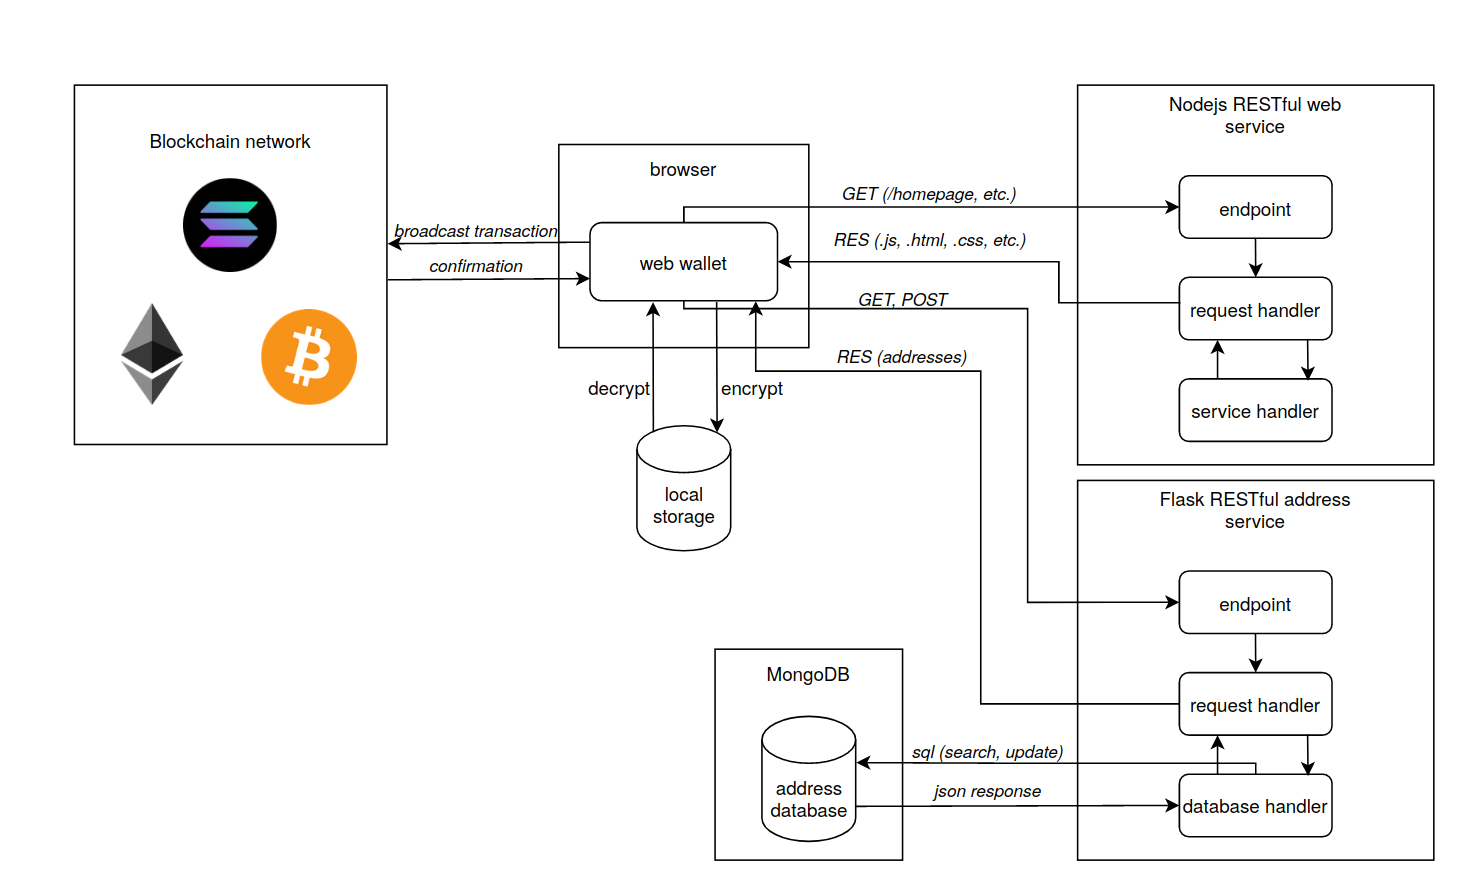
\includegraphics[width=1\textwidth]{images/ecosystem.png}
    \caption[Overview of entire system]{Overview of entire system}
    \label{fig:eco}
\end{figure}

The user can access our web wallet through their web browser from any platform. Features and detail of every page will be presented in Section \ref{webui}. After creating the wallet, the master secret seed will be saved in their local storage with the index paths  (for convenience). The master seed should be encrypted with the user’s password for safety since there are attacks aimed at browser sensitive information. We will discuss all potential attacks in Chapter \ref{chap:testing}.


Every time the user derives a new child, the wallet will access the local storage to get (decrypt) the secret seed then generate the expected keys. The exact process happens when the user needs to transfer assets. The secret seed will be accessed to get the private key for the digital signature generation.


\subsection{Address service}

\label{address}
\subsubsection{Technologies}

The address service provides API for public wallet management and searching (in transaction). We apply Flask framework and MongoDB for our module. The system contains the total of four API.

\bigskip
{\textbf{Flask}}. Flask \cite{grinberg2018flask} is a micro web framework written in python. It is classified as a microframework because it does not require particular tools or libraries. It has no database abstraction layer, form validation, or any other components where pre-existing third-party libraries provide standard functions. However, Flask supports extensions that can add application features as if they were implemented in Flask itself. Extensions exist for object-relational mappers, form validation, upload handling, various open authentication technologies, and several standard framework-related tools. We also use Flask since python is more comfortable dealing with JSON content-type requests.


\bigskip
{\textbf{MongoDB}}. MongoDB \cite{mongo} is a source-available cross-platform document-oriented database program. Classified as a NoSQL database program, MongoDB uses JSON-like documents with optional schemas, so it is suitable for our database design.

\bigskip
\subsubsection{API Provider}

For reference only, the base URL of the system is http://localhost:8080.

{\textbf{Get address}}. Request for the list of receiver address (who also use our HD wallet) on a specific blockchain. The response contains information of purpose of those wallet and the addresses.

Request:

\begin{framed}
    POST http://localhost:8080/getaddress
\end{framed}

\begin{tabular}{m{3cm}  m{9cm} m{2.6cm}}
    \toprule
    Field & Description & Format                                            \\ 
    \midrule
    address & The SHA512 hash of the master address of receiver wallet. & Text   \\ 
    chain   & The ID of the blockchain (see in BIP44 \cite{bip44}) & Text    \\ 
    \bottomrule
\end{tabular}
% \captionof{table}{\label{Tab:IMP-1} Get address request components.}
\bigskip

Example request:

\begin{framed}
\hspace*{13mm}    curl - - request POST \par
\hspace*{13mm}        - - url http://localhost:8080/getaddress \par
\hspace*{13mm}        - - header 'Content-Type: application/json' \par
\hspace*{13mm}        - - data '\{ \par
\hspace*{20mm}                "address": "test", \par
\hspace*{20mm}                "chain": "501" \par
\hspace*{20mm}            \}' \par
\end{framed}


Example response:

\begin{framed}
    \hspace*{13mm}        \{\par
    \hspace*{13mm}          "list\_address": \{ \par
    \hspace*{18mm}        "default": "childaddress", \par
    \hspace*{18mm}        "business": "childaddress1"    \par
    \hspace*{18mm}        \},\par
    \hspace*{13mm}                "message": "Succeed",   \par
    \hspace*{13mm}                "status": "Succeed",  \par
    \hspace*{13mm}             "statusCode": 200   \par
    \hspace*{13mm}                 \}    \par

\end{framed}
    
\bigskip
{\textbf{Create default Wallet}}
\bigskip

Request to publish the address to the server. The web will automatically call this service when a wallet is created (the one default child’s index is 2021). The response contains confirmation of the request.

Request:

\begin{framed}
    POST http://localhost:8080/createdefault
\end{framed}

\begin{tabular}{m{3cm}  m{9cm} m{2.6cm} }
    \toprule
    Field & Description & Format                                            \\ 
    \midrule
    \_id & The value of the SHA512(master address) of the HD wallet. This is also the \_id field of MongoDB document schema.  & Text   \\ 
    address   & The dictionary of default generated addresses & Text    \\ 
    \bottomrule
\end{tabular}
% \captionof{table}{\label{Tab:IMP-2} Create default Wallet request components.}
\bigskip

Example request:

\begin{framed}
\hspace*{13mm}    curl - - request POST \par
\hspace*{13mm}        - - url http://localhost:8080/createdefault \par
\hspace*{13mm}        - - header 'Content-Type: application/json' \par
\hspace*{13mm}        - - data '\{ \par
\hspace*{20mm}                "\_id": "tess1231",\par
\hspace*{27mm}                "address": \{ \par
\hspace*{35mm}                "1": \{ \par
\hspace*{40mm}                "default": "wallet1" \{ \par
\hspace*{40mm}                \}, \par
\hspace*{35mm}                "60": \{ \par
\hspace*{40mm}                "default": "wallet2" \par
\hspace*{40mm}                \}, \par
\hspace*{35mm}                "501": \{ \par
\hspace*{40mm}                "default": "wallet3" \par
\hspace*{40mm}                \} \par
\hspace*{27mm}              \} \par
\hspace*{20mm}            \}' \par
\end{framed}

Example response:

\begin{framed}
    \hspace*{13mm}        \{ \par
    \hspace*{13mm}                "message": "Succeed",    \par
    \hspace*{13mm}                "status": "Succeed",    \par
    \hspace*{13mm}             "statusCode": 200    \par
    \hspace*{13mm}                 \}    \par
\end{framed}


\bigskip
{\textbf{Push child address}}
\bigskip

Request to append a child address to existed address list on the server. The response contains confirmation of the request.

Request:

\begin{framed}
    POST http://localhost:8080/pushaddress
\end{framed}

\begin{tabular}{ m{3cm}  m{9cm}  m{2.6cm} }
    \toprule
    Field & Description & Format                                            \\ 
    \midrule
    \_id & The value of the SHA512(master address) of the HD wallet. This is also the \_id field of MongoDB document schema.  & Text   \\ 
    chain   & The ID of the blockchain & Text    \\ 
    purpose   & The purpose of this child wallet & Text    \\ 
    child\_address   & The address of the child wallet & Text    \\ 
    \bottomrule
\end{tabular}
% \captionof{table}{\label{Tab:IMP-3} Push child address to database.}
\bigskip

Example request:

\begin{framed}
\hspace*{13mm}    curl - - request POST \par
\hspace*{13mm}        - - url http://localhost:8080/pushaddress \par
\hspace*{13mm}        - - header 'Content-Type: application/json' \par
\hspace*{13mm}        - - data '\{ \par
\hspace*{27mm}                "address": "test",  \par
\hspace*{40mm}                "chain": "60", \par
\hspace*{40mm}                "purpose": "business1", \par
\hspace*{40mm}                "child\_address": " 0x88d696674a104489f..." \par
\hspace*{27mm}              \} \par
\end{framed}

Example response:

\begin{framed}
    \hspace*{13mm}        \{ \par
    \hspace*{13mm}                "message": "Succeed",    \par
    \hspace*{13mm}                "status": "Succeed",    \par
    \hspace*{13mm}             "statusCode": 200    \par
    \hspace*{13mm}                 \}    \par
\end{framed}


\bigskip
{\textbf{Pull child address }}
\bigskip

Request to delete a child address that existed on the server. The response contains confirmation of the request.

Request:

\begin{framed}
    POST http://localhost:8080/deleteaddress
\end{framed}

\begin{tabular}{m{3cm} m{9cm}  m{2.6cm}}
    \toprule
    Field & Description & Format                                            \\ 
    \midrule
    \_id & The value of the SHA512(master address) of the HD wallet. This is also the \_id field of MongoDB document schema.  & Text   \\ 
    chain   & The ID of the blockchain & Text    \\ 
    purpose   & The purpose of this child wallet & Text    \\ 
    child\_address   & The address of the child wallet & Text    \\ 
    \bottomrule

\end{tabular}
% \captionof{table}{\label{Tab:IMP-4} Push child address to database.}
\bigskip

Example request:

\begin{framed}
\hspace*{13mm}    curl - - request POST \par
\hspace*{13mm}        - - url http://localhost:8080/deleteaddress \par
\hspace*{13mm}        - - header 'Content-Type: application/json' \par
\hspace*{13mm}        - - data '\{ \par
\hspace*{27mm}                "address": "test",  \par
\hspace*{40mm}                "chain": "60", \par
\hspace*{40mm}                "purpose": "business1", \par
\hspace*{40mm}                "child\_address": " 0x88d696674a104489f..." \par
\hspace*{27mm}              \} \par
\end{framed}

Example response:

\begin{framed}
    \hspace*{13mm}        \{ \par
    \hspace*{13mm}                "message": "Succeed",    \par
    \hspace*{13mm}                "status": "Succeed",    \par
    \hspace*{13mm}             "statusCode": 200    \par
    \hspace*{13mm}                 \}    \par
\end{framed}

There are potential attacks on this kind of server since we haven’t provided any authentication at all. We discuss these attacks in the evaluation Section (see Chapter \ref{fig:testcase}).

\subsection{Web Wallet Service}
\label{webui}

\bigskip
{\textbf{React JS}}. React was invented by a software engineer at Facebook named Jordan Walke, was first introduced in 2011. Walke finalized the prototype and created React in 2012, soon combined it into Facebook in the same year. In 2013 React became open-source and later became available in Ruby on Rails and Python Applications. This is followed by the release of React Native, an extension of React for mobile development on Android and iOS, in 2015. Since then, React consistently pushed out many releases throughout the years, enhancing and submitting new features for users. React is a versatile tool that can be operated on both desktop and mobile platforms with many different features. One of them is the ability to produce interactively rather than simple static pages that can update and rerender data after each input from the user, thus permitting for a seamless UI without refreshing the whole page every time a component is changed. The reason for this is that React’s structure is based on components that allow for the design of complex UIs due to the component logic being written in JavaScript.

There are another framework for JavaScript such as Vue.js, Angular, etc, but we choose React as it the most popular one. Compared to other framework, React is just a library, not a pre-built framework, which is easier to configure and develop. Another difference is that, React uses multiple components together to build up a website rather than a website template and update its inner elements. Each component is an HTML element which has its own properties and state. For this reason, React allows re-rendering specific components of the webpage in comparison to Vue.js or Angular, which re-renders a whole page. The reason why it can work like that is because React does not update the DOM directly, but through a virtual DOM. The virtual DOM is a JavaScript object which stores all the information to create a DOM. Every time a component updates its state, the virtual DOM compares the change and only render the changes onto the DOM. Overall, React helps us to maintain and update code easier through the component structure (similar to Object-oriented programming style), interactive website, and efficient DOM manipulation with virtual DOM.

\bigskip
{\textbf{Node.js}}. Node.js is required as it provides a JavaScript environment and libraries for developing React. Node.js is an open-source, cross-platform, back-end JavaScript runtime environment that runs on the V8 engine and executes JavaScript code outside a web browser. Node.js lets developers use JavaScript to write command line tools and for server-side scripting—running scripts server-side to produce dynamic web page content before the page is sent to the user's web browser. Consequently, Node.js represents a "JavaScript everywhere" paradigm, unifying web-application development around a single programming language, rather than different languages for server-side and client-side scripts.

\bigskip
{\textbf{User Interface}}
\bigskip

We implement our design and create our web pages as follow:

\begin{figure}[h!]
    \centering
    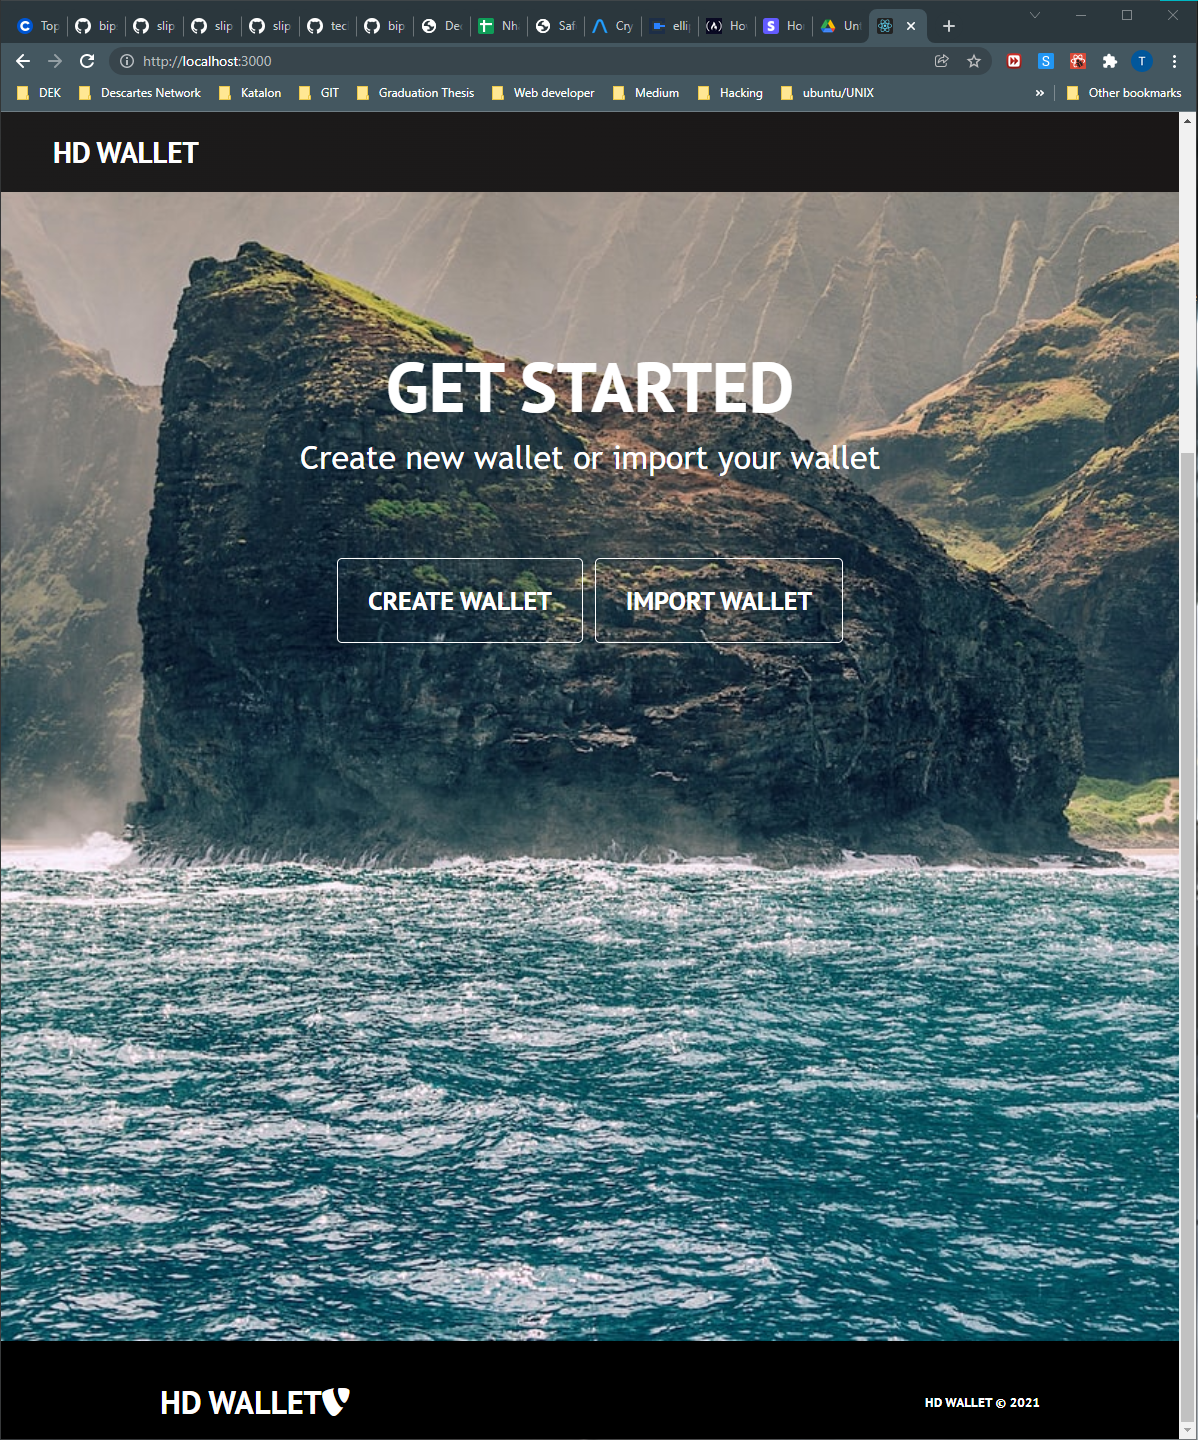
\includegraphics[width=1\textwidth]{images/Homepage.png}
    \caption[Homepage]{Homepage}
    \label{fig:homepage}
  \end{figure}


  \begin{figure}[h!]
    \centering
    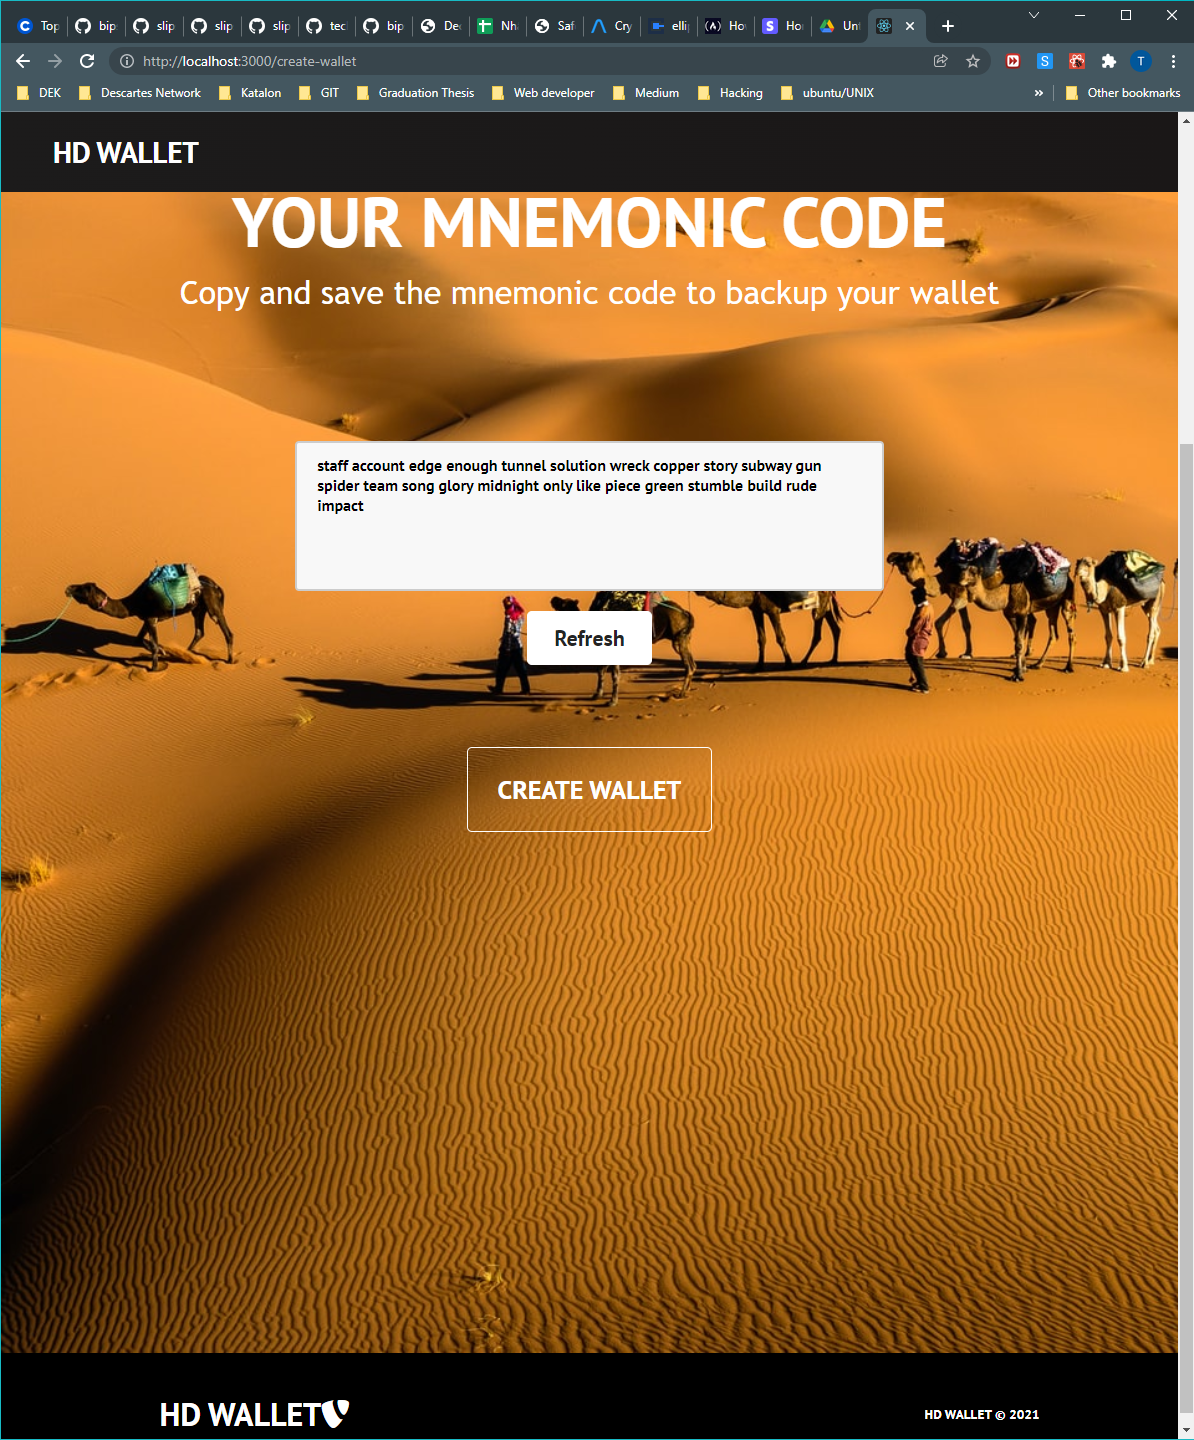
\includegraphics[width=1\textwidth]{images/CreateWallet.png}
    \caption[Create wallet page]{Create wallet page}
    \label{fig:createwallet}
  \end{figure}


  \begin{figure}[h!]
    \centering
    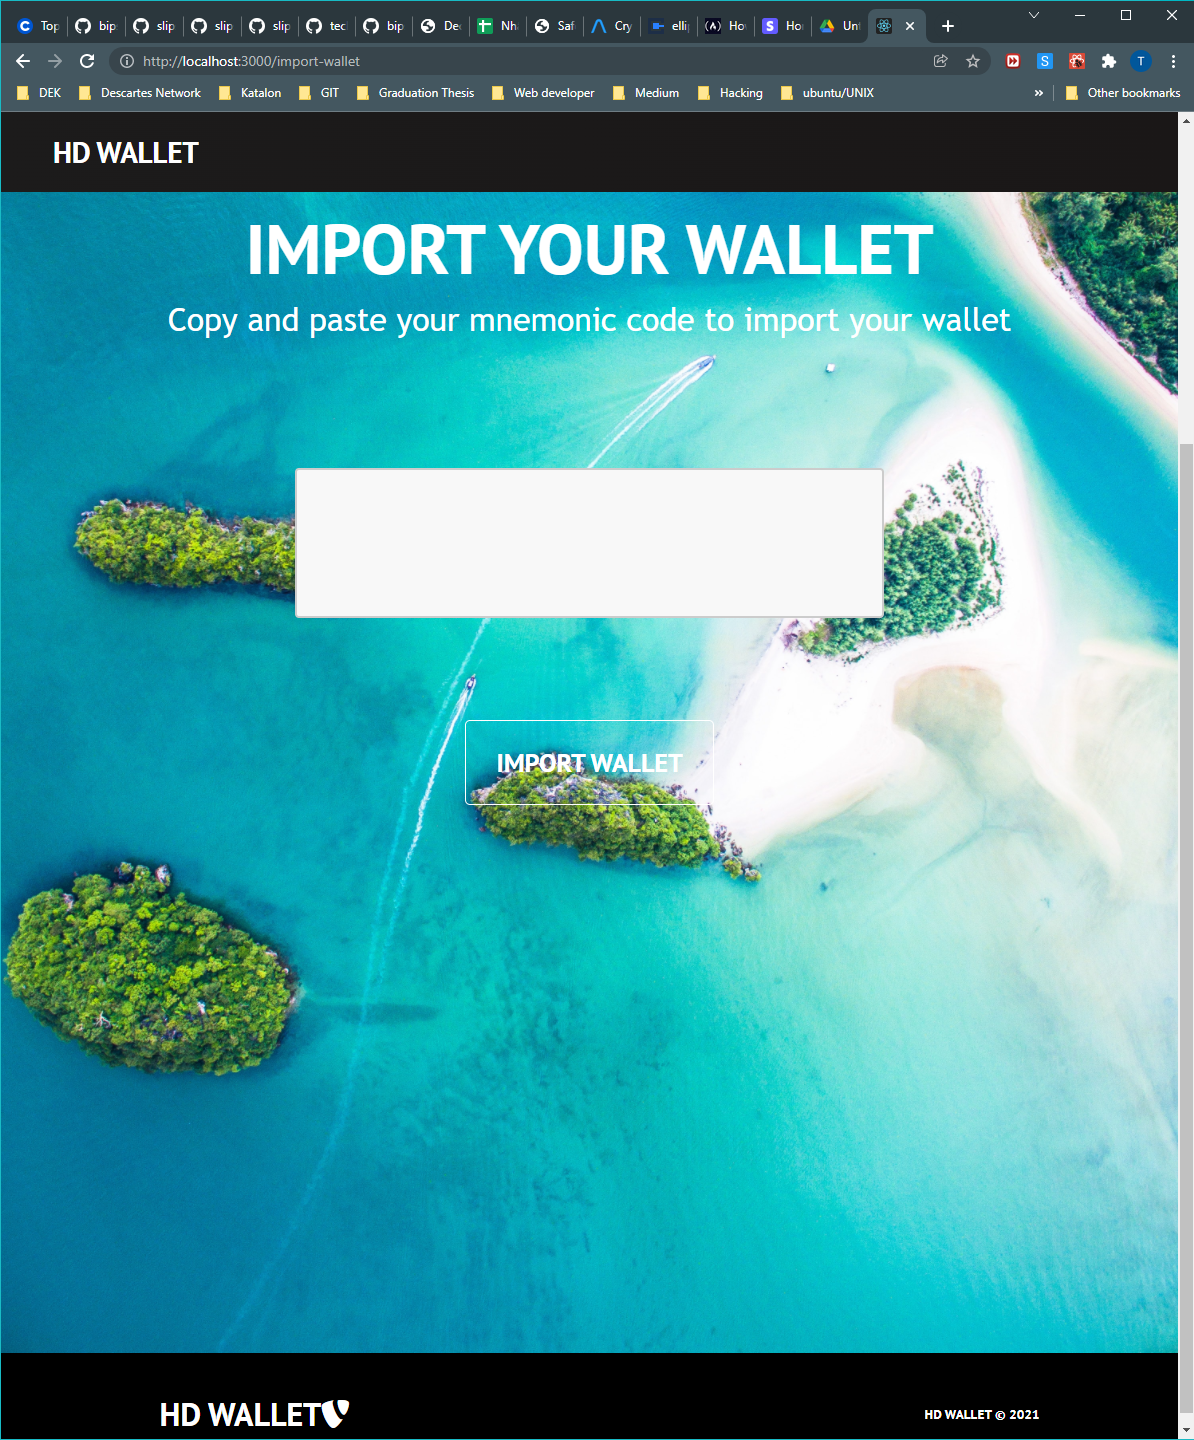
\includegraphics[width=1\textwidth]{images/ImportWallet.png}
    \caption[Import wallet page]{Import wallet page}
    \label{fig:importwallet}
  \end{figure}

  \begin{figure}[h!]
    \centering
    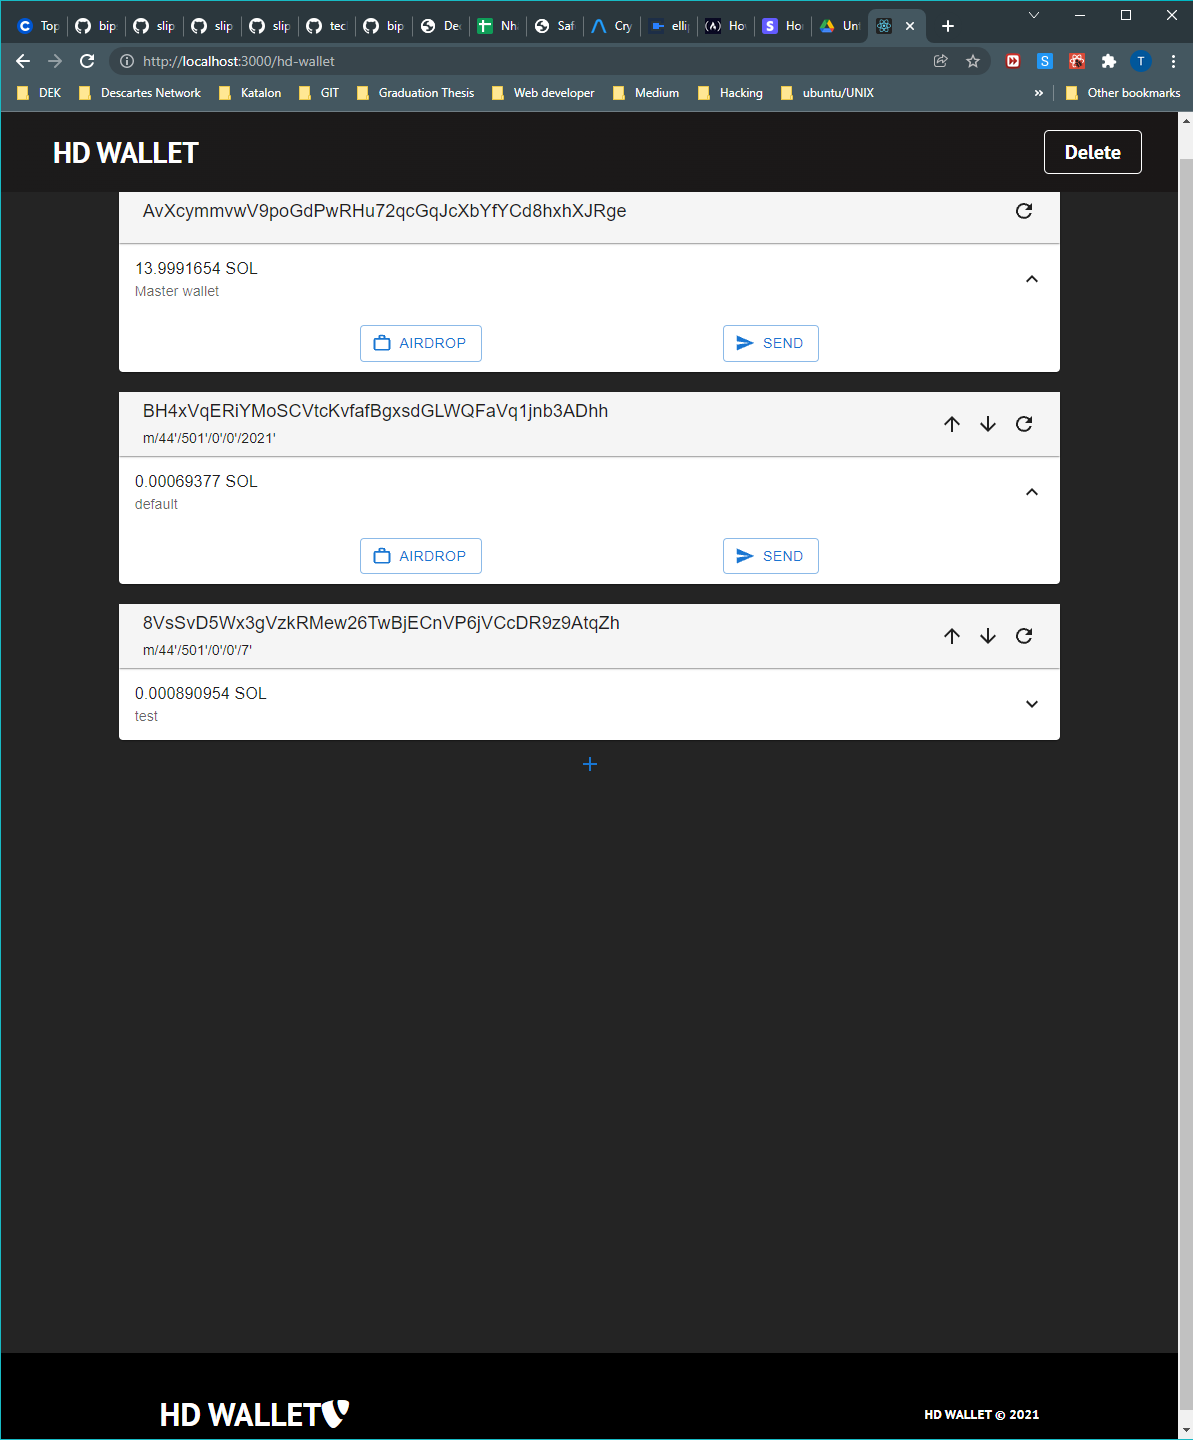
\includegraphics[width=1\textwidth]{images/Mainpage.png}
    \caption[Wallet page]{Wallet page}
    \label{fig:wallet}
  \end{figure}

  \begin{figure}[h!]
    \centering
    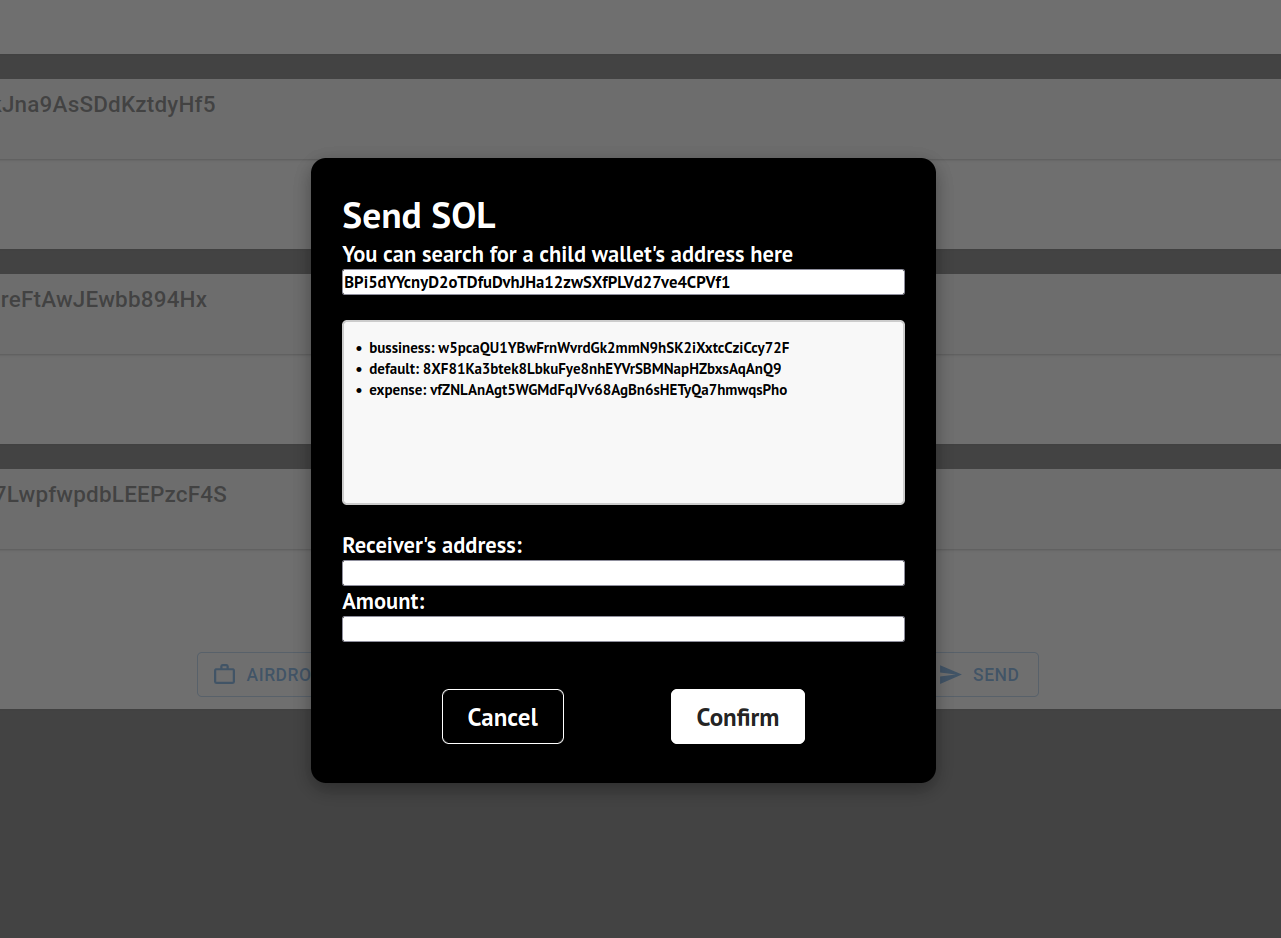
\includegraphics[width=1\textwidth]{images/search.png}
    \caption[Transaction and search]{Transaction and search}
    \label{fig:transactionandsearch}
  \end{figure}


  \begin{figure}[h!]
    \centering
    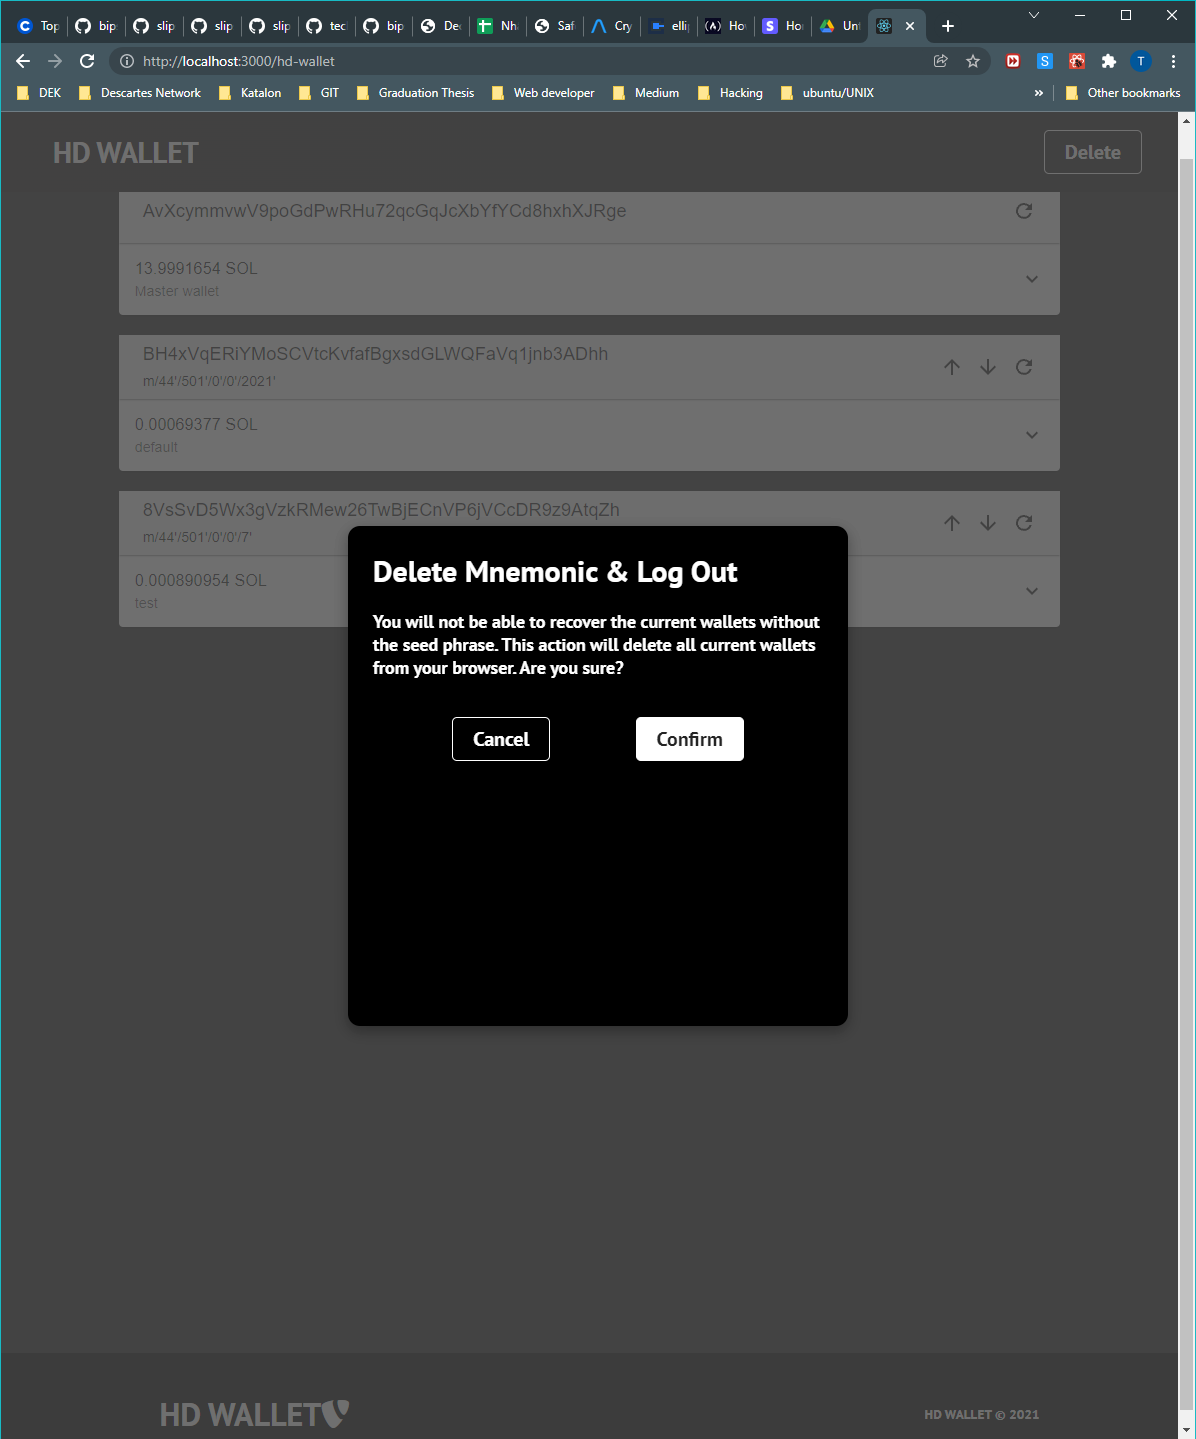
\includegraphics[width=1\textwidth]{images/DeleteMnemonic.png}
    \caption[Delete wallet]{Delete wallet}
    \label{fig:delwallet}
  \end{figure}
